\chapter{Digitale Zertifikate und \texorpdfstring{\acrshort{PKI}}{PKI}}\label{chap:zertifikate-pki}

Im vorangegangenen Kapitel haben wir gesehen, wie digitale Signaturen mit asymmetrischen Kryptosystemen (wie \gls{RSA}) erstellt und überprüft werden können. Eine mathematisch korrekte Signatur garantiert jedoch nur die Integrität der Nachricht und dass sie mit dem zum öffentlichen Schlüssel passenden privaten Schlüssel erzeugt wurde. Sie beantwortet noch nicht die fundamentale Vertrauensfrage der Praxis: \emph{Gehört der öffentliche Schlüssel tatsächlich der Person oder Institution, für die sie sich ausgibt?}

\section{Das Vertrauensproblem in der Praxis}
Eine digitale Signatur beweist mathematisch zwei zentrale Eigenschaften:
\begin{itemize}
	\item \textbf{Integrität:} Die Nachricht wurde auf dem Übertragungsweg nicht manipuliert (jede Veränderung führt zu einem anderen Hashwert und macht die Signatur ungültig).
	\item \textbf{Authentizität:} Die Signatur konnte nur mit dem privaten Schlüssel erzeugt werden, der zum angegebenen öffentlichen Schlüssel gehört.
\end{itemize}

\paragraph*{Das Problem: Wessen Signatur ist es wirklich?}
Hier stösst die reine Mathematik an eine praktische Grenze: \emph{Woher weiss der Empfänger (Bob), dass ein bestimmter öffentlicher Schlüssel tatsächlich Alice gehört?}

Ein Angreifer (Eve) könnte ein eigenes Schlüsselpaar erzeugen und den öffentlichen Schlüssel unter dem Namen von Alice oder als angebliche Webseite einer Bank veröffentlichen. Signiert Eve anschliessend eine gefälschte Nachricht mit ihrem eigenen privaten Schlüssel, so bestätigt die mathematische Überprüfung mit Eves öffentlichem Schlüssel formal die Gültigkeit der Signatur. Bob wiegt sich in falscher Sicherheit, da er die Signatur nicht der echten Identität zuordnen kann (Man-in-the-Middle-Angriff).

\paragraph*{Praxisnahe Lösung: Digitale Zertifikate und \texorpdfstring{\acrshort{PKI}}{PKI}}
Um das Vertrauensproblem in der Praxis zu lösen (beispielsweise beim sicheren Surfen via \gls{HTTPS} und \gls{TLS} oder bei der elektronischen Signatur), wird eine sogenannte \textbf{Public-Key-Infrastruktur} (\gls{PKI}) eingesetzt:
\begin{itemize}
	\item \textbf{Zertifizierungsstellen (\emph{Certificate Authorities}, \glspl{CA}):} Unabhängige, staatlich oder industriell anerkannte Organisationen prüfen vor der Schlüsselausgabe die reale Identität der antragstellenden Person oder Institution.
	\item \textbf{Digitale Zertifikate:} Die \gls{CA} stellt ein standardisiertes Dokument (Zertifikat) aus, welches den öffentlichen Schlüssel an die Identität (z.\,B.\ den Domainnamen \texttt{www.beispiel.ch}) bindet. Dieses Zertifikat wird von der \gls{CA} mit deren eigenem privaten Schlüssel signiert.
	\item \textbf{Vertrauensanker (Root-\glspl{CA}):} Betriebssysteme und Browser besitzen eine vorinstallierte Liste vertrauenswürdiger Stammzertifikate. Wird eine Verbindung aufgebaut, prüft die Software automatisch die Signaturkette (\emph{Certificate Chain}) bis zu einem vertrauenswürdigen Stammzertifikat.
\end{itemize}
Erst das Zusammenspiel aus kryptographischer Signatur und einer funktionierenden Vertrauensinfrastruktur ermöglicht verlässliche Sicherheit in modernen Kommunikationsnetzen (siehe \cref{fig:pki-ablauf}).

\begin{figure}[H]
	\centering
	\begin{tikzpicture}[
	scale=0.78, every node/.style={transform shape},
	actor/.style={rectangle, rounded corners, draw=black, fill=gray!15, minimum width=3.4cm, minimum height=1.1cm, font=\bfseries, align=center, inner sep=4pt},
	stepbox/.style={rectangle, rounded corners, draw=#1, fill=#1!8, line width=0.8pt, font=\small, align=center, inner sep=6pt},
	msgarrow/.style={->, >=stealth, line width=1pt, #1},
	badge/.style={circle, fill=#1, text=white, font=\bfseries\footnotesize, inner sep=2pt}
]
	% Spaltenkoordinaten
	\def\colA{0}     % Alice
	\def\colCA{5.5}  % CA
	\def\colB{11}    % Bob

	% --- AKTEURE (Kopfzeile) ---
	\node[actor] (alice) at (\colA, 0) {Alice\\{\footnotesize (Absenderin)}\\[2pt]{\scriptsize öff.: $(e_A, n_A)$,\; priv.: $d_A$}};
	\node[actor, fill=DarkOrchid!15, draw=DarkOrchid] (ca) at (\colCA, 0) {\textcolor{DarkOrchid}{\faCertificate{}} CA\\{\footnotesize (Zertifizierungsstelle)}\\[2pt]{\scriptsize öff.: $(e_{\text{CA}}, n_{\text{CA}})$,\; priv.: $d_{\text{CA}}$}};
	\node[actor] (bob) at (\colB, 0) {Bob\\{\footnotesize (Empfänger)}\\[2pt]{\scriptsize vorinstalliert: $(e_{\text{CA}}, n_{\text{CA}})$}};

	% Vertikale Hilfslinien
	\draw[dashed, gray!40] (alice.south) -- (\colA, -13.8);
	\draw[dashed, gray!40] (ca.south) -- (\colCA, -5.8);
	\draw[dashed, gray!40] (bob.south) -- (\colB, -13.8);

	% --- PHASE 1: ZERTIFIZIERUNG (VORAB) ---
	\node[font=\footnotesize\bfseries\color{DarkOrchid!80!black}, fill=white, inner sep=2pt] at (\colCA, -1.1) {Phase 1: Zertifikatserstellung (einmalig vorab)};

	% Pfeil 1: Alice -> CA (Schlüsselregistrierung)
	\node[badge=RoyalBlue] (b1) at (\colA+0.6, -2.0) {1};
	\draw[msgarrow=RoyalBlue] (b1.east) -- (\colCA-0.3, -2.0)
		node[midway, above=2pt, font=\footnotesize] {Antrag mit Daten $z = (\text{\enquote{Alice}}, e_A, n_A)$};

	% CA signiert
	\node[stepbox=DarkOrchid] (ca_sign) at (\colCA, -3.4) {
		\textbf{CA prüft Identität \& signiert $z$:}\\
		$\text{Cert}_A := z^{d_{\text{CA}}} \bmod n_{\text{CA}}$
	};

	% Pfeil 2: CA -> Alice (Zertifikatsausgabe)
	\node[badge=DarkOrchid] (b2) at (\colCA-0.6, -4.8) {2};
	\draw[msgarrow=DarkOrchid] (b2.west) -- (\colA+0.3, -4.8)
		node[midway, above=2pt, font=\footnotesize] {Ausgabe: Zertifikat $(z, \text{Cert}_A)$};

	% --- PHASE 2: VERSAND DER SIGNIERTEN NACHRICHT ---
	\node[font=\footnotesize\bfseries\color{RoyalBlue!80!black}, fill=white, inner sep=2pt] at (5.5, -6.0) {Phase 2: Signieren \& Übertragen};

	% Alice signiert
	\node[stepbox=RoyalBlue] (alice_sign) at (\colA, -7.3) {
		\textbf{Alice signiert Vertrag $m$:}\\
		$s := m^{d_A} \bmod n_A$
	};

	% Pfeil 3: Alice -> Bob
	\node[badge=black] (b3) at (\colA+1.8, -9.0) {3};
	\draw[msgarrow=black] (b3.east) -- (\colB-1.8, -9.0)
		node[midway, above=3pt, font=\footnotesize, align=center] {Vertrag $m$ \quad+\quad Signatur $s$ \quad+\quad Zertifikat $(z, \text{Cert}_A)$};

	% --- PHASE 3: ZWEISTUFIGE VERIFIKATION BEI BOB ---
	\node[font=\footnotesize\bfseries\color{ForestGreen!80!black}, fill=white, inner sep=2pt] at (\colB, -10.3) {Phase 3: Verifikation bei Bob};

	% Bob Verifikation
	\node[stepbox=ForestGreen] (bob_verify) at (\colB, -12.1) {
		\textbf{Schritt A: Zertifikat mit $(e_{\text{CA}}, n_{\text{CA}})$ prüfen}\\
		$z' := (\text{Cert}_A)^{e_{\text{CA}}} \bmod n_{\text{CA}}$\\
		$\rightarrow \text{Gilt } z' = z\text{?} \implies (e_A, n_A)\text{ ist echt!}$\\[4pt]
		\textbf{Schritt B: Signatur mit $(e_A, n_A)$ prüfen}\\
		$m' := s^{e_A} \bmod n_A$\\
		$\rightarrow \text{Gilt } m' = m\text{?} \implies \text{Vertrag ist echt!} \textcolor{ForestGreen}{\mathbf{\checkmark}}$
	};
\end{tikzpicture}

	\caption{Zweistufige Vertrauenskette digitaler Zertifikate (\acrshort{PKI})}
	\label{fig:pki-ablauf}
\end{figure}

\begin{myremark}[Wozu nützen Signaturen, wenn sich jeder ein Zertifikat holen kann?]
	Eine häufige Frage lautet: \emph{Wenn sich jeder beliebig ein Zertifikat von einer \gls{CA} ausstellen lassen kann, wo liegt dann der Sicherheitsgewinn?}

	Der entscheidende Unterschied ist: Jeder kann sich ein Zertifikat für seine \textbf{eigene} Identität beziehungsweise Domain ausstellen lassen -- aber eben \textbf{nicht} für die eines anderen.

	In einer \gls{PKI} kommen dabei \textbf{zwei verschiedene Signaturen} auf zwei Ebenen zum Einsatz:
	\begin{enumerate}
		\item \textbf{Die Zertifizierungsstelle signiert ein Zertifikat:} Die \gls{CA} bestätigt mit ihrem privaten Schlüssel verbindlich die Zuordnung eines öffentlichen Schlüssels zu einer bestimmten Domain (oder Person). Dafür muss der Antragsteller der \gls{CA} nachweisen, dass er diese Domain tatsächlich kontrolliert.
		\item \textbf{Der Besitzer signiert mit seinem privaten Schlüssel:} Mit dem im Zertifikat beglaubigten öffentlichen Schlüssel kann jedermann auf der Welt prüfen, ob die Signatur passt und ob die signierten Daten unverändert sind.
	\end{enumerate}

	\smallskip\noindent\textbf{Konkretes Beispiel:}
	Ein Angreifer kann sich problemlos ein gültiges Zertifikat für seine eigene Domain wie \texttt{meine-fake-bank.ch} ausstellen lassen. Damit kann er jedoch:
	\begin{itemize}
		\item \textbf{weder} im Browser als \texttt{ubs.com} auftreten (da ihm keine anerkannte \gls{CA} ein Zertifikat für eine fremde Domain ausstellt),
		\item \textbf{noch} Signaturen erzeugen, die zum öffentlichen Schlüssel der echten \texttt{ubs.com} passen (da er deren privaten Schlüssel nicht besitzt).
	\end{itemize}

	\smallskip\noindent\textbf{Wichtiges Missverständnis -- Gültig $\neq$ Vertrauenswürdig:}
	Ein gültiges Zertifikat bedeutet \textbf{nicht}: \enquote{\emph{Dieser Anbieter ist vertrauenswürdig und ehrlich}}, sondern ausschliesslich: \enquote{\emph{Dieser öffentliche Schlüssel gehört nachweislich zu dieser Domain}}. Auch eine betrügerische Phishing-Website kann völlig legal ein gültiges Zertifikat für ihre eigene Betrugsdomain besitzen.

	Der Vorteil von \gls{RSA}-Signaturen liegt genau in dieser Asymmetrie: Alle dürfen prüfen, aber ausschliesslich der Besitzer des privaten Schlüssels kann die passende Signatur erzeugen. Die Zertifizierungsstelle hilft zusätzlich dabei, zweifelsfrei zu wissen, \emph{wessen} Schlüssel man zum Prüfen verwendet.
\end{myremark}

\begin{myexercise}[Ablauf einer zertifizierten digitalen Signatur in der Praxis]
	Alice möchte einen wichtigen Vertrag digital an Bob senden. Um sicherzustellen, dass Bob der Signatur vertrauen kann, nutzt Alice ein digitales Zertifikat einer vertrauenswürdigen Zertifizierungsstelle (\gls{PKI}/\gls{CA}).
	
	Folgende Schlüssel existieren:
	\begin{itemize}
		\item \textbf{Zertifizierungsstelle (\gls{CA}):} Öffentlicher Schlüssel $(e_{\text{CA}}, n_{\text{CA}})$ (auf Bobs Computer vorinstalliert), privater Schlüssel $d_{\text{CA}}$.
		\item \textbf{Alice:} Öffentlicher Schlüssel $(e_A, n_A)$, privater Schlüssel $d_A$.
		\item \textbf{Angreiferin (Eve):} Öffentlicher Schlüssel $(e_E, n_E)$, privater Schlüssel $d_E$.
	\end{itemize}
	
	\begin{enumerate}
		\item \textbf{Zertifikatserstellung:} Welche Formel berechnet die \gls{CA}, um aus den Antragsdaten $z = (\text{\enquote{Alice}}, e_A, n_A)$ das signierte Zertifikat $\text{Cert}_A$ zu erzeugen?
		\item \textbf{Nachrichtenversand:} Welche Formel berechnet Alice zur Erzeugung der Signatur $s$ für den Vertrag $m$? Welche Daten überträgt sie an Bob?
		\item \textbf{Zweistufige Überprüfung durch Bob:} Welche beiden konkreten Rechnungen führt Bobs Computer aus, um nacheinander die Echtheit des Zertifikats und die Echtheit der Nachricht nachzuweisen?
		\item \textbf{Angriffsszenario:} Eve fängt die Nachricht ab, verändert den Vertrag und signiert ihn mit ihrem eigenen privaten Schlüssel $d_E$. Warum scheitert dieser Angriff bei Bob?
	\end{enumerate}
	\begin{myanswer}
		\begin{enumerate}
			\item Die \gls{CA} signiert die Antragsdaten $z$ mit ihrem privaten Schlüssel $d_{\text{CA}}$:\\
			      $\text{Cert}_A = z^{d_{\text{CA}}} \bmod n_{\text{CA}}$.
			\item Alice signiert den Vertrag $m$ mit ihrem privaten Schlüssel $d_A$:\\
			      $s = m^{d_A} \bmod n_A$.\\
			      Sie sendet an Bob: den Vertrag $m$, ihre Signatur $s$ und das Zertifikat $(z, \text{Cert}_A)$.
			\item Bobs Computer führt zwei modulare Berechnungen durch:
			      \begin{enumerate}
				      \item \textbf{Zertifikatsprüfung:} Er prüft die \gls{CA}-Signatur mit dem vorinstallierten öffentlichen \gls{CA}-Schlüssel:\\
				            $z' = (\text{Cert}_A)^{e_{\text{CA}}} \bmod n_{\text{CA}}$.\\
				            Gilt $z' = z$, gehört der enthaltene Schlüssel $(e_A, n_A)$ garantiert Alice.
				      \item \textbf{Signaturprüfung:} Er prüft die Signatur mit dem verifizierten Schlüssel $(e_A, n_A)$:\\
				            $m' = s^{e_A} \bmod n_A$.\\
				            Gilt $m' = m$, ist der Vertrag unverfälscht und stammt von Alice.

			      \end{enumerate}
			\item Eve besitzt kein von der \gls{CA} signiertes Zertifikat auf ihren Namen. Sendet sie ihr eigenes Schlüsselpaar $(e_E, n_E)$ mit, schlägt die Zertifikatsprüfung mit $(e_{\text{CA}}, n_{\text{CA}})$ fehl. Verwendet sie Alices Zertifikat mit $(e_A, n_A)$, schlägt die Signaturprüfung mit $s = m^{d_E} \bmod n_E$ fehl, da $s^{e_A} \not\equiv m \pmod{n_A}$.
		\end{enumerate}
	\end{myanswer}
\end{myexercise}

\section{Die Zertifikatkette in der Praxis: Vertrauenskaskade}
In der Praxis signiert eine oberste Zertifizierungsstelle (\textbf{Root-\gls{CA}}) fast nie direkt einzelne Webserver-Zertifikate. Das weltweite Vertrauensmodell basiert stattdessen auf einer mehrstufigen \textbf{Zertifikatkette} (\emph{Certificate Chain}, siehe \cref{fig:certificate-chain}):

\begin{enumerate}
	\item \textbf{Root-\gls{CA} (Stammzertifizierungsstelle):} Unbedingter Vertrauensanker (\emph{Trust Anchor}). Ihr selbstsigniertes Zertifikat ist fest im \textbf{Trust Store} des Betriebssystems oder Browsers vorinstalliert. Ihr privater Schlüssel wird streng isoliert offline aufbewahrt (\emph{Air-Gapped} in Hardware-Sicherheitsmodulen, \glspl{HSM}) und nur selten für Zwischenzertifikate aktiviert.
	\item \textbf{Intermediate-\gls{CA} (Zwischenzertifizierungsstelle):} Wird von der Root-\gls{CA} signiert und führt das operative Tagesgeschäft der Zertifikatsausstellung durch.
	\item \textbf{Server- / Blatt-Zertifikat (\emph{Leaf Certificate}):} Das eigentliche Zertifikat der Domain (z.\,B.\ \texttt{www.sbb.ch}), signiert von der Intermediate-\gls{CA}.
\end{enumerate}

\paragraph*{Sicherheitsvorteil der Kaskade}
Müsste die Root-\gls{CA} jedes Serverzertifikat signieren, wäre ihr privater Schlüssel permanent auf internetverbundenen Servern exponiert. Bei einem Schlüsselverlust einer Intermediate-\gls{CA} widerruft die Root-\gls{CA} lediglich dieses eine Zwischenzertifikat (via Zertifikatssperrlisten \glspl{CRL} oder Statusabfrage \gls{OCSP}). Das in Milliarden Endgeräten verankerte Root-Zertifikat bleibt unangetastet.

\begin{figure}[H]
	\centering
	\begin{tikzpicture}[
	scale=0.82, every node/.style={transform shape},
	box/.style={rectangle, rounded corners=4pt, draw=#1, fill=#1!10, line width=1pt, align=center, inner sep=5pt, font=\small},
	chainarrow/.style={->, >=stealth, line width=1.1pt, #1}
]
	% Hierarchie-Knoten
	\node[box=DarkOrchid, minimum width=9.5cm] (root) at (0, 3.6) {
		\textbf{\textcolor{DarkOrchid}{\faKey{} Root-CA: \texttt{Amazon Root CA 1} / \texttt{SwissSign Gold CA - G2}}}\\
		{\scriptsize \faShield*{} Vorinstalliert im Trust Store $\cdot$ Privater Schlüssel offline (Air-Gapped)}
	};

	\node[box=RoyalBlue, minimum width=9.5cm] (inter) at (0, 1.8) {
		\textbf{\textcolor{RoyalBlue}{\faCertificate{} Intermediate-CA: \texttt{Amazon RSA 2048 M04} / \texttt{Swiss Government PKI}}}\\
		{\scriptsize Signiert von der Root-CA $\cdot$ Operative Zertifikatsausgabe}
	};

	\node[box=ForestGreen, minimum width=9.5cm] (leaf) at (0, 0.0) {
		\textbf{\textcolor{ForestGreen}{\faServer{} Server-Zertifikat: \texttt{www.sbb.ch} / \texttt{www.admin.ch}}}\\
		{\scriptsize Signiert von der Intermediate-CA $\cdot$ Öffentlicher Schlüssel der Website}
	};

	\node[box=gray, minimum width=9.5cm, fill=gray!8] (client) at (0, -1.8) {
		\textbf{\faLaptop{} Webbrowser / Betriebssystem (Client)}\\
		{\scriptsize Prüft Signaturkette von unten nach oben bis zum vorinstallierten Root-Zertifikat}
	};

	% Pfeile (Signaturfluss von oben nach unten)
	\draw[chainarrow=DarkOrchid] (root.south) -- (inter.north)
		node[midway, right=6pt, font=\footnotesize] {signiert Zwischenzertifikat};
	\draw[chainarrow=RoyalBlue] (inter.south) -- (leaf.north)
		node[midway, right=6pt, font=\footnotesize] {signiert Server-Zertifikat};
	\draw[chainarrow=ForestGreen] (leaf.south) -- (client.north)
		node[midway, right=6pt, font=\footnotesize] {überträgt Zertifikatkette bei \gls{HTTPS}};

	% Prüfpfeil rückwärts links
	\draw[->, >=stealth, dashed, line width=1.1pt, BrickRed] (client.west) to[out=168, in=192] node[midway, left=4pt, font=\scriptsize\bfseries, align=center, rotate=90] {Kryptographische Verifikation} (root.west);

\end{tikzpicture}

	\caption{Hierarchische Zertifikatkette (Vertrauenskaskade)}
	\label{fig:certificate-chain}
\end{figure}

\paragraph*{Schweizer Vertrauensdienste (\texorpdfstring{\acrshort{ZertES}}{ZertES})}
In der Schweiz regelt das \textbf{Bundesgesetz über die elektronische Signatur (\gls{ZertES})} die rechtliche Gleichstellung qualifizierter elektronischer Signaturen mit der eigenhändigen Unterschrift (Art.~14 Abs.~$2^{\text{bis}}$ OR). Anerkannte Schweizer Vertrauensdienste sind unter anderem \textbf{SwissSign} (Schweizerische Post / SwissID), \textbf{Swisscom Trust Services} und \textbf{SWITCHpki} (für Schweizer Hochschulen und Schulen).

\paragraph*{Zertifikatsprüfung im Webbrowser}
Beim Aufruf einer \gls{HTTPS}-Website (z.\,B.\ \url{https://www.sbb.ch}) übermittelt der Server die gesamte Kette (Server- und Zwischenzertifikat). Der Browser prüft jede Signatur rückwärts bis zur Root-\gls{CA} im lokalen Trust Store.

\begin{itemize}
	\item \textbf{Safari (macOS):} Menü \textbf{Safari $\rightarrow$ Details zur Verbindungssicherheit\dots} (siehe \cref{fig:safari-certificate-sbb}).
	\item \textbf{Chrome / Edge:} Klick auf das \textbf{Schieberegler-Symbol} (\emph{Tune-Icon}) links der \gls{URL} $\rightarrow$ \emph{Verbindung ist sicher} $\rightarrow$ \emph{Zertifikat ist gültig} (oder via Entwicklertools \texttt{F12} $\rightarrow$ \emph{Security}).
	\item \textbf{Firefox:} Klick auf das \textbf{Schloss-Symbol} links der \gls{URL} $\rightarrow$ \emph{Sichere Verbindung} $\rightarrow$ \emph{Weitere Informationen} $\rightarrow$ \emph{Zertifikat anzeigen}.
\end{itemize}

\begin{figure}[H]
	\centering
	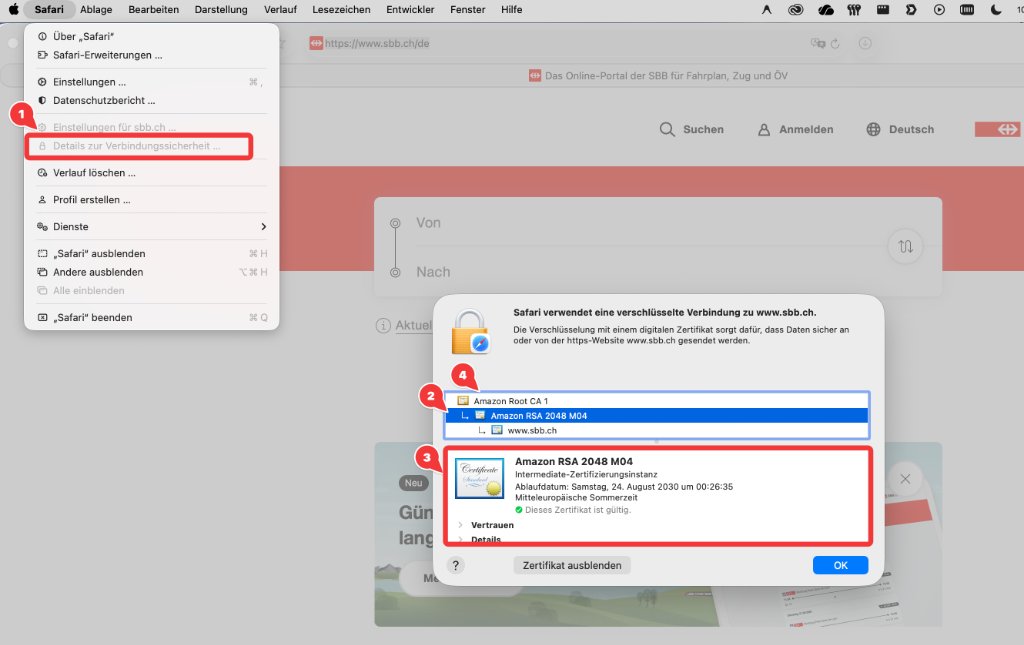
\includegraphics[width=0.88\linewidth]{Grundlagen_Info/03_Kryptologie/Figures/certificate_hierarchy_sbb}
	\caption{Zertifikatsinspektion in Apple Safari (\texttt{www.sbb.ch}):
		\textbf{(1)} Menüaufruf;
		\textbf{(2)} Dreistufige Hierarchie (\texttt{Amazon Root CA 1} $\rightarrow$ \texttt{Amazon RSA 2048 M04} $\rightarrow$ \texttt{www.sbb.ch});
		\textbf{(3)} Gültigkeitsdetails der Intermediate-\gls{CA};
		\textbf{(4)} Status der \gls{TLS}-Verschlüsselung.}
	\label{fig:safari-certificate-sbb}
\end{figure}

\begin{myremark}[Wer betreibt Root-CAs? Von Tech-Giganten bis zu Staaten]
	Dass beim Aufruf von \texttt{sbb.ch} ein Technologiekonzern wie \emph{Amazon} als Root-\gls{CA} auftaucht, wirft eine naheliegende Frage auf: Warum sind Stammzertifizierungsstellen nicht ausschliesslich staatliche Behörden?
	
	Die Web-\gls{PKI} ist historisch dezentral gewachsen. Wer als Root-\gls{CA} anerkannt wird, entscheiden primär die Betreiber der Betriebssysteme und Browser (Apple, Google, Microsoft, Mozilla) im Rahmen des internationalen \emph{CA/Browser Forums}. Jede Root-\gls{CA} muss jährlich strenge, unabhängige Sicherheitsaudits (z.\,B.\ \emph{WebTrust}) nachweisen.
	
	In der Praxis unterscheidet man vier Hauptarten von Zertifizierungsstellen:
	\begin{itemize}
		\item \textbf{Cloud- \& Tech-Konzerne (z.\,B.\ Amazon Trust Services, Google Trust Services):} Betreiben eigene \glspl{PKI}, um Millionen von Servern und Kunden ihrer Cloud-Plattformen (wie \gls{AWS}) automatisiert und kostengünstig abzusichern.
		\item \textbf{Kommerzielle Vertrauensdienste (z.\,B.\ DigiCert, SwissSign):} Unabhängige Sicherheitsunternehmen, deren Kerngeschäft in der Ausstellung und Identitätsprüfung für Dritte liegt.
		\item \textbf{Gemeinnützige Initiativen (z.\,B.\ \emph{Let's Encrypt}):} Stellen kostenlose, automatisierte Zertifikate für jedermann bereit und sichern heute über die Hälfte des weltweiten Webverkehrs ab.
		\item \textbf{Staatliche \glspl{PKI} (z.\,B.\ \emph{Swiss Government PKI}):} Dienen hoheitlichen Behördennetzen, eGovernment, Identitätskarten und qualifizierten elektronischen Signaturen gemäss \gls{ZertES}.
	\end{itemize}
	
	\smallskip\noindent\textbf{Warum nutzt die SBB Amazon und nicht die Bundes-\gls{PKI}?}
	Die SBB betreibt ihre Web-Infrastruktur auf \gls{AWS} (mit automatisierter Zertifikatsverwaltung). Zudem ist die bundeseigene \emph{Swiss Government PKI} eine interne Behörden-\gls{PKI} und nicht in weltweiten Standard-Browsern vorinstalliert; ihr Einsatz auf öffentlichen Webseiten würde bei Fahrgästen Zertifikatswarnungen auslösen.
\end{myremark}

\begin{myexercise}[Zertifikats-Detektiv im Webbrowser]
	Öffnen Sie einen Webbrowser Ihrer Wahl (Safari, Chrome, Edge oder Firefox) und rufen Sie eine Schweizer Website auf, z.\,B.\ das Portal der Schweizerischen Bundesbahnen (\url{https://www.sbb.ch}), der Schweizer Bundesverwaltung (\url{https://www.admin.ch}) oder Ihrer Kantonsschule.
	
	\begin{enumerate}
		\item Öffnen Sie über das jeweilige Browsermenü die Zertifikatsinformationen.
		\item Welche Zertifikate bilden die Hierarchiekette von der obersten Root-\gls{CA} über Zwischenzertifikate bis zum Blatt-Zertifikat der Webseite?
		\item Notieren Sie für das Blatt-Zertifikat:
		      \begin{itemize}
			      \item Den gemeinsamen Namen (\emph{Common Name}, \gls{CN}) bzw.\ die Domain.
			      \item Die Gültigkeitsdauer (von / bis).
			      \item Den verwendeten Algorithmus und die Schlüssellänge für den öffentlichen Schlüssel (z.\,B.\ \gls{RSA} 2048 Bit oder \gls{ECC} P-256).
			      \item Den verwendeten Hash-Algorithmus der Signatur (z.\,B.\ \gls{SHA}-256).
		      \end{itemize}
		\item \textbf{Denkaufgabe:} Warum haben moderne Server-Zertifikate typischerweise nur noch eine kurze Gültigkeitsdauer von maximal 398 Tagen (bzw.\ oft nur 90 Tagen wie bei \emph{Let's Encrypt}), während Root-Zertifikate oft für 20 bis 30 Jahre ausgestellt werden?
	\end{enumerate}
	\begin{myanswer}
		\begin{enumerate}
			\setcounter{enumi}{1}
			\item Beispielhafte Kette für \texttt{www.sbb.ch} (gemäss \cref{fig:safari-certificate-sbb}):
			      \begin{itemize}
				      \item \textbf{Root-\gls{CA}:} \texttt{Amazon Root CA 1}
				      \item \textbf{Intermediate-\gls{CA}:} \texttt{Amazon RSA 2048 M04}
				      \item \textbf{Server-Zertifikat:} \texttt{www.sbb.ch}
			      \end{itemize}
			\item Typische Werte:
			      \begin{itemize}
				      \item \textbf{\gls{CN}:} \texttt{www.sbb.ch} (Inhaberin: Schweizerische Bundesbahnen SBB)
				      \item \textbf{Gültigkeit:} Typischerweise 1 Jahr (bzw.\ bis zum angegebenen Ablaufdatum).
				      \item \textbf{Öffentlicher Schlüssel:} \gls{RSA} (2048 Bit) bzw.\ \gls{ECC} (256 Bit).
				      \item \textbf{Signatur-Hash:} \gls{SHA}-256 mit \gls{RSA}-Verschlüsselung (\texttt{sha256WithRSA}).
			      \end{itemize}
			\item Kurze Laufzeiten bei Serverzertifikaten begrenzen das Zeitfenster für den Missbrauch, falls ein privater Serverschlüssel unbemerkt gestohlen wird. Zudem zwingen kurze Laufzeiten Administratoren zu automatisierten Erneuerungsprozessen und ermöglichen einen schnellen Wechsel zu sichereren kryptographischen Standards. Root-Zertifikate hingegen müssen jahrzehntelang gültig sein, da ihre Erneuerung ein manuelles Update von Milliarden Betriebssystemen und Firmware-Chips weltweit erfordert.
		\end{enumerate}
	\end{myanswer}
\end{myexercise}
